% Chapter 5
\chapter{DATA ANALYSIS} % Write in your own chapter title

The data stored at the remote server are subjected to analysis with the goal of discovering useful information, suggesting conclusion and supporting decision making. There are different ways of analysing data. These ways are briefly described here.

\subsection{Time series}
A single variable is captured over a period of time, such as the unemployment rate over a 10-year period. A line chart may be used to demonstrate the trend. This is shown in Figure \ref{fig:time}

\begin{figure}[h!]
	\centering
	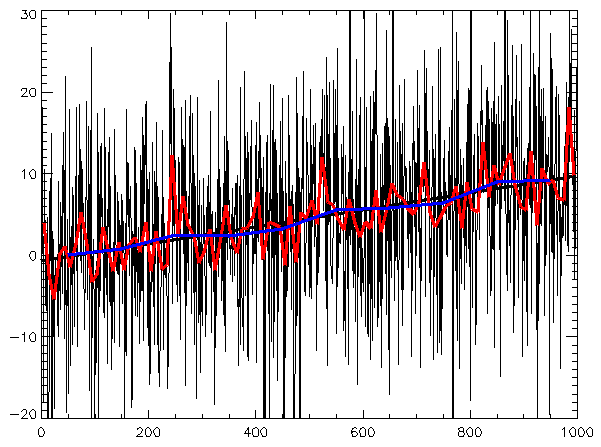
\includegraphics[scale=0.3]{time}
	\caption{Time series}
	\label{fig:time}
\end{figure}

\subsection{Correlation}
Comparison between observations represented by two variables (X,Y) to determine if they tend to move in the same or opposite directions. For example, plotting unemployment (X) and inflation (Y) for a sample of months. A scatter plot as shown in Figure \ref{fig:scatter} is typically used for this message.

\begin{figure}[h!]
	\centering
	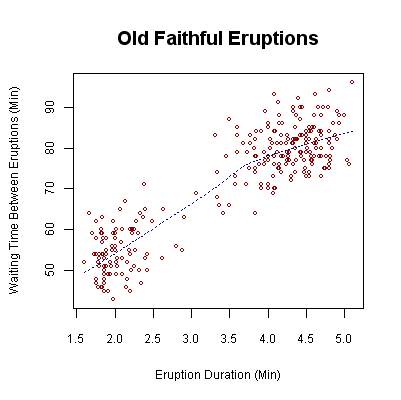
\includegraphics[scale=0.4]{scatter}
	\caption{Scatter plot}
	\label{fig:scatter}
\end{figure}

\newpage
\subsection{Analytical Activities of the Data Users}
Users may have particular data points of interest within a data set, such low-level user analytic activities are given below

\begin{table}[!ht]
	\centering
	\begin{tabular}{| m{4em} | m{6em}| m{7em} | m{8em} |} 
		\hline
		\textbf{Task} & \textbf{General description} & \textbf{Abstract} & \textbf{Examples} \\ 
		\hline
		Retrieve value & Find attributes from a set & What are values of attributes in data cases & Name of victim\\ 
		\hline
		Compute derived values & Compute an aggregate numeric representation & What is value of aggregate function F over a set S of cases? & What is the average number of accidents ? \\ 
		\hline
		Find extremum & Find extreme values in data cases & What are the top/bottom data w.r.t attribute A? & Type of vehicles involved in frequent accidents \\
		\hline
		Sort & Given a set of data cases, rank them according to some ordinal metric & What is the sorted order of a set S of data cases according to value of attribute A? & Order accident based on time \\
		\hline
	\end{tabular}
	\caption{Types of analytics}
\end{table}